\documentclass[12pt,a4paper]{article}
\usepackage[UTF8]{ctex}
\usepackage{amsmath, amssymb}
\usepackage{geometry}
\usepackage{booktabs}
\usepackage{graphicx}
\usepackage{float}
\geometry{left=2.5cm, right=2.5cm, top=2.5cm, bottom=2.5cm}
\title{\textbf{问题二 灵敏度分析报告}\\[4pt]
\large VLSI 布图规划设计 --- 参数灵敏度分析}
\author{2026 年第七届"华数杯"大学生数学建模竞赛 B 题}
\date{2026/08}
\begin{document}
\maketitle

\section{S1：精修初始温度除数 t2-div 灵敏度}

精修阶段初始温度 $T_0/\text{t2-div}$ 控制局部搜索的"冷热"程度。
扫描 t2-div $\in [20, 70]$（三芯片各 9 点），各值取 HPWL 最小。

\begin{figure}[H]
\centering
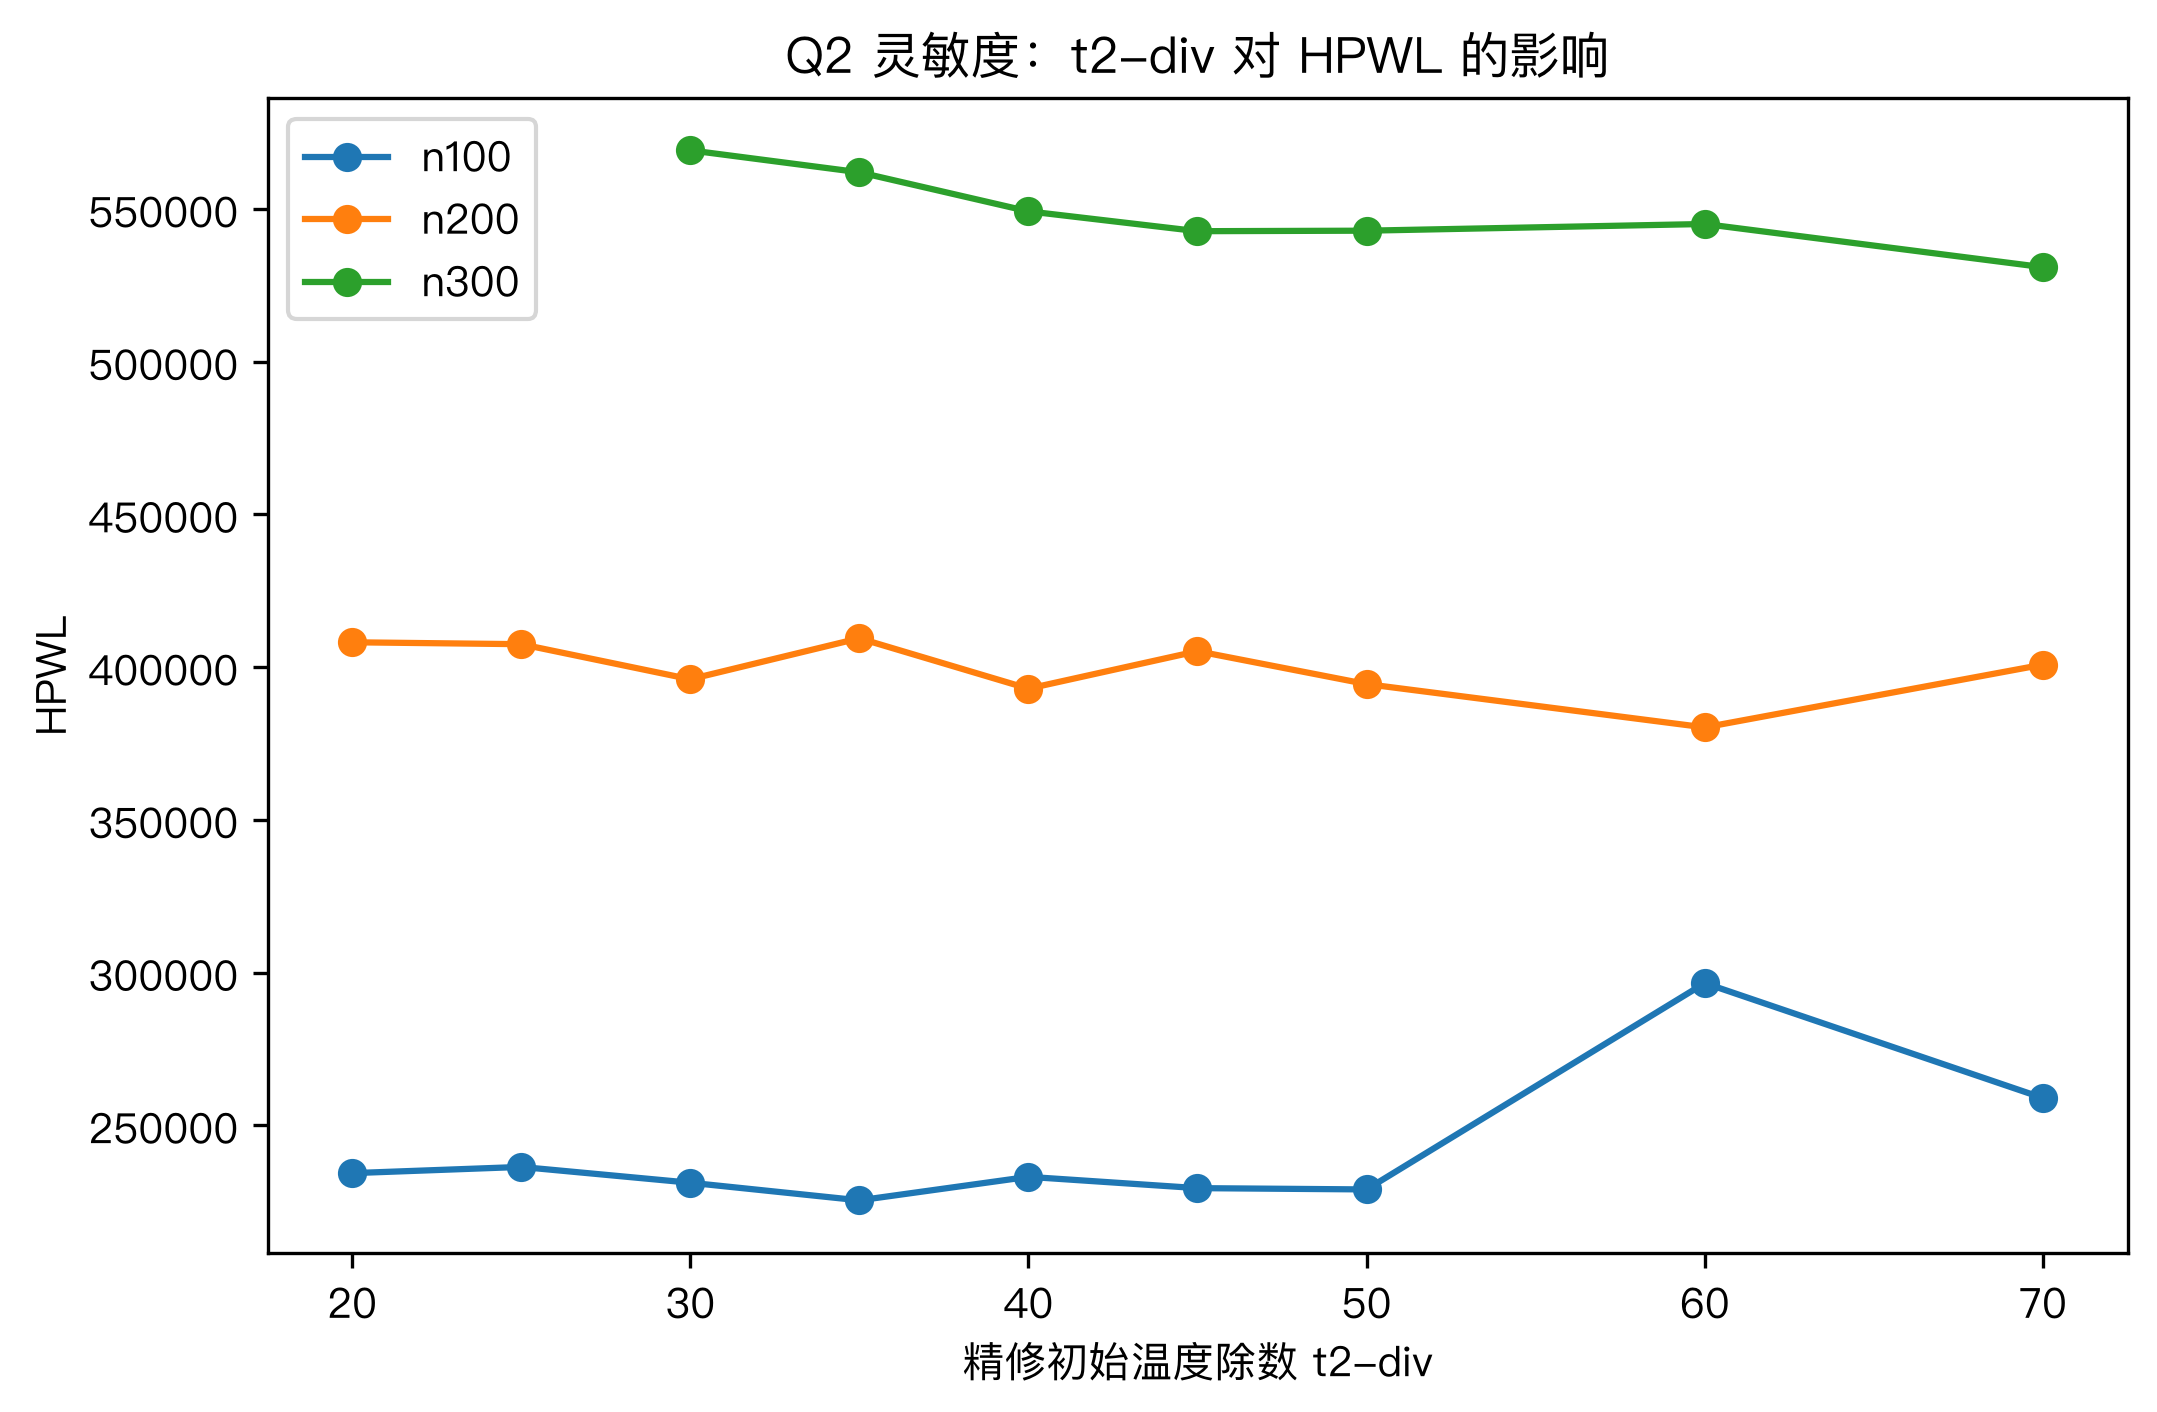
\includegraphics[width=0.82\textwidth]{../../做图/q2_t2div_sensitivity.png}
\caption{HPWL 随 t2-div 变化}
\end{figure}

  \begin{table}[H]
  \centering
  \caption{S1 数据（HPWL 最小）}\label{tab:q2s1}
  \begin{tabular}{lll}
  \toprule
  chip & t2\_div & hpwl \\
  \midrule
  n100 & 20 & 234304.5 \\
  n100 & 25 & 236341.0 \\
  n100 & 30 & 231169.0 \\
  n100 & 35 & 225403.5 \\
  n100 & 40 & 233093.0 \\
  n100 & 45 & 229397.0 \\
  n100 & 50 & 228974.0 \\
  n100 & 60 & 296532.0 \\
  n100 & 70 & 258899.5 \\
  n200 & 20 & 408126.0 \\
  n200 & 25 & 407502.5 \\
  n200 & 30 & 396024.0 \\
  n200 & 35 & 409441.5 \\
  n200 & 40 & 392945.0 \\
  n200 & 45 & 405209.5 \\
  n200 & 50 & 394435.0 \\
  n200 & 60 & 380261.0 \\
  n200 & 70 & 400805.5 \\
  n300 & 30 & 569205.0 \\
  n300 & 35 & 562019.0 \\
  n300 & 40 & 549225.5 \\
  n300 & 45 & 542730.0 \\
  n300 & 50 & 542895.0 \\
  n300 & 60 & 545087.0 \\
  n300 & 70 & 530944.5 \\
  \bottomrule
  \end{tabular}
  \end{table}

\textbf{结论}：最优 t2-div \textbf{随芯片漂移}——n100 谷底在 35
（225404），n200 谷底在 60（380261），n300 谷底在 70（530944，扫描
边界，参数定稿阶段加密 80/90 确认）。固定全局 t2-div 会损失
4$\sim$6\% 的 HPWL 收益，故交付按芯片独立取参；t2-div 过大
（$\ge 60$，n100）或过小（$\le 25$）均明显劣化。

\section{S2：死区比例灵敏度}

死区比例 $d$ 决定轮廓边长 $\text{side} = \lceil \sqrt{\Sigma A(1+d)}\rceil$，
扫描 $d \in [0.10, 0.18]$（n100/n200）。

\begin{figure}[H]
\centering
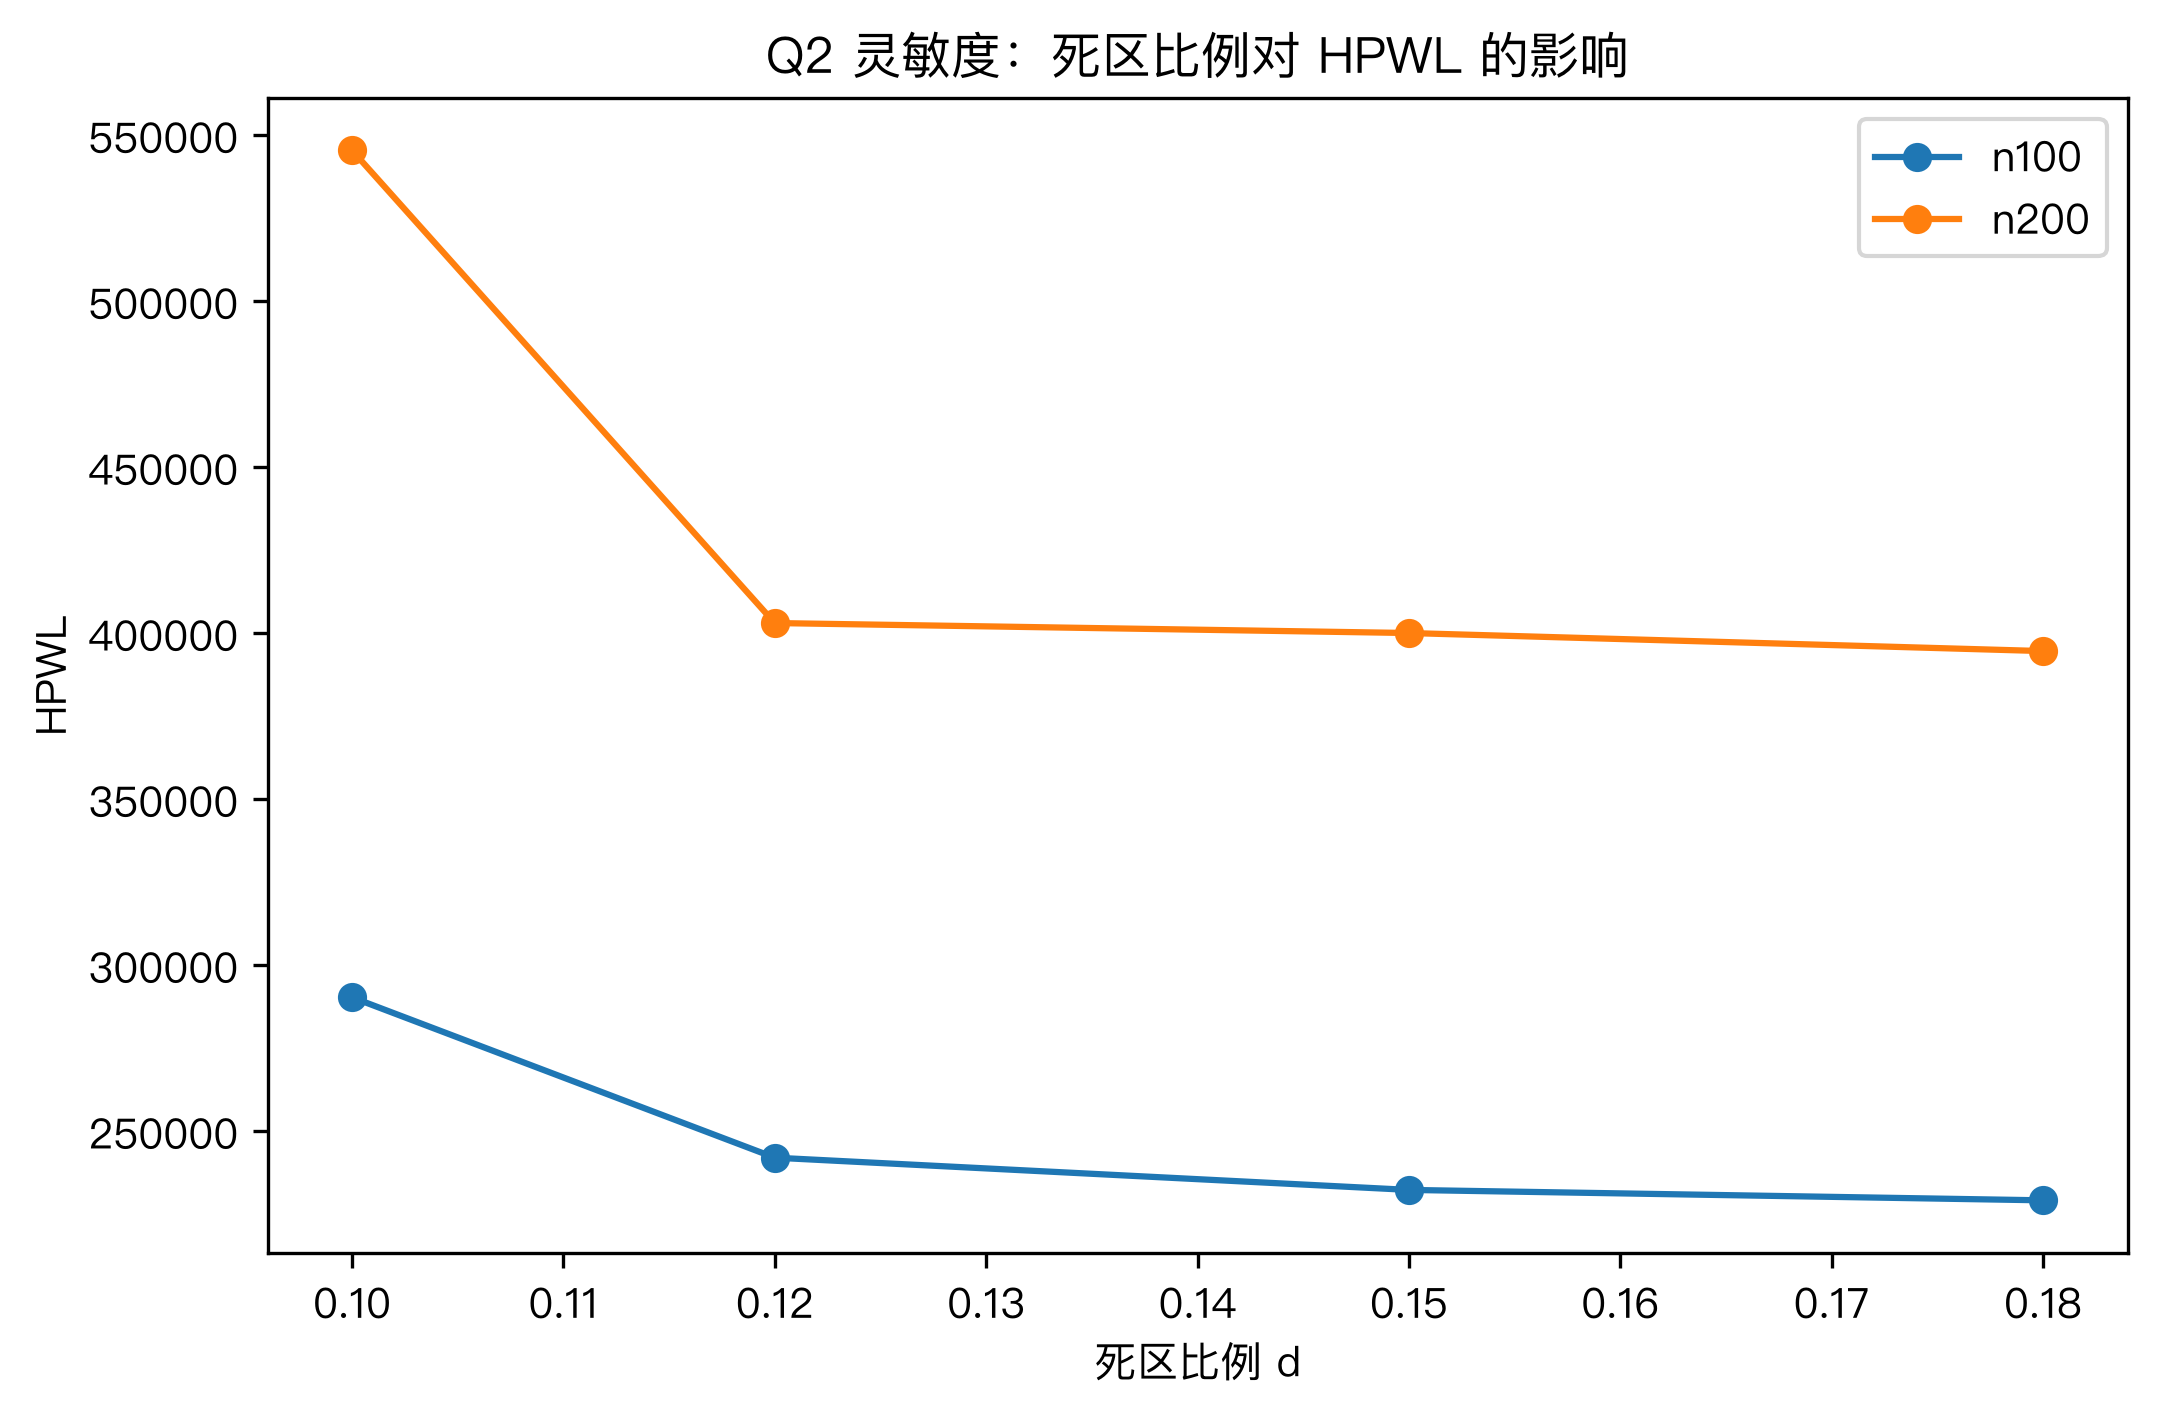
\includegraphics[width=0.82\textwidth]{../../做图/q2_dead_ratio_sensitivity.png}
\caption{HPWL 随死区比例变化}
\end{figure}

  \begin{table}[H]
  \centering
  \caption{S2 数据}\label{tab:q2s2}
  \begin{tabular}{lll}
  \toprule
  chip & dead & hpwl \\
  \midrule
  n100 & 0.1 & 290127.0 \\
  n100 & 0.12 & 241826.5 \\
  n100 & 0.15 & 232114.0 \\
  n100 & 0.18 & 228974.0 \\
  n200 & 0.1 & 545280.0 \\
  n200 & 0.12 & 402880.0 \\
  n200 & 0.15 & 399874.0 \\
  n200 & 0.18 & 394435.0 \\
  \bottomrule
  \end{tabular}
  \end{table}

\textbf{结论}：HPWL 随 $d$ 增大\textbf{单调改善}（轮廓越宽松、布线空间
越大）：$d$ 从 0.10 增至 0.18，n100 HPWL 下降 21\%、n200 下降 28\%；
其中 $d \le 0.12$ 区间恶化显著（n200 达 545280）。基准 $d=0.15$ 落在
平稳区，对 $d$ 的 $\pm 0.03$ 波动不敏感（变化 $<1.5\%$）——说明基准
选择稳健，也为问题 3 的 $d^*$ 搜索提供边界参照。

\section{S3：轮次收敛灵敏度}

在 t2-div=50 下扫描 repeats $= 12/16/20/24/32$。

\begin{figure}[H]
\centering
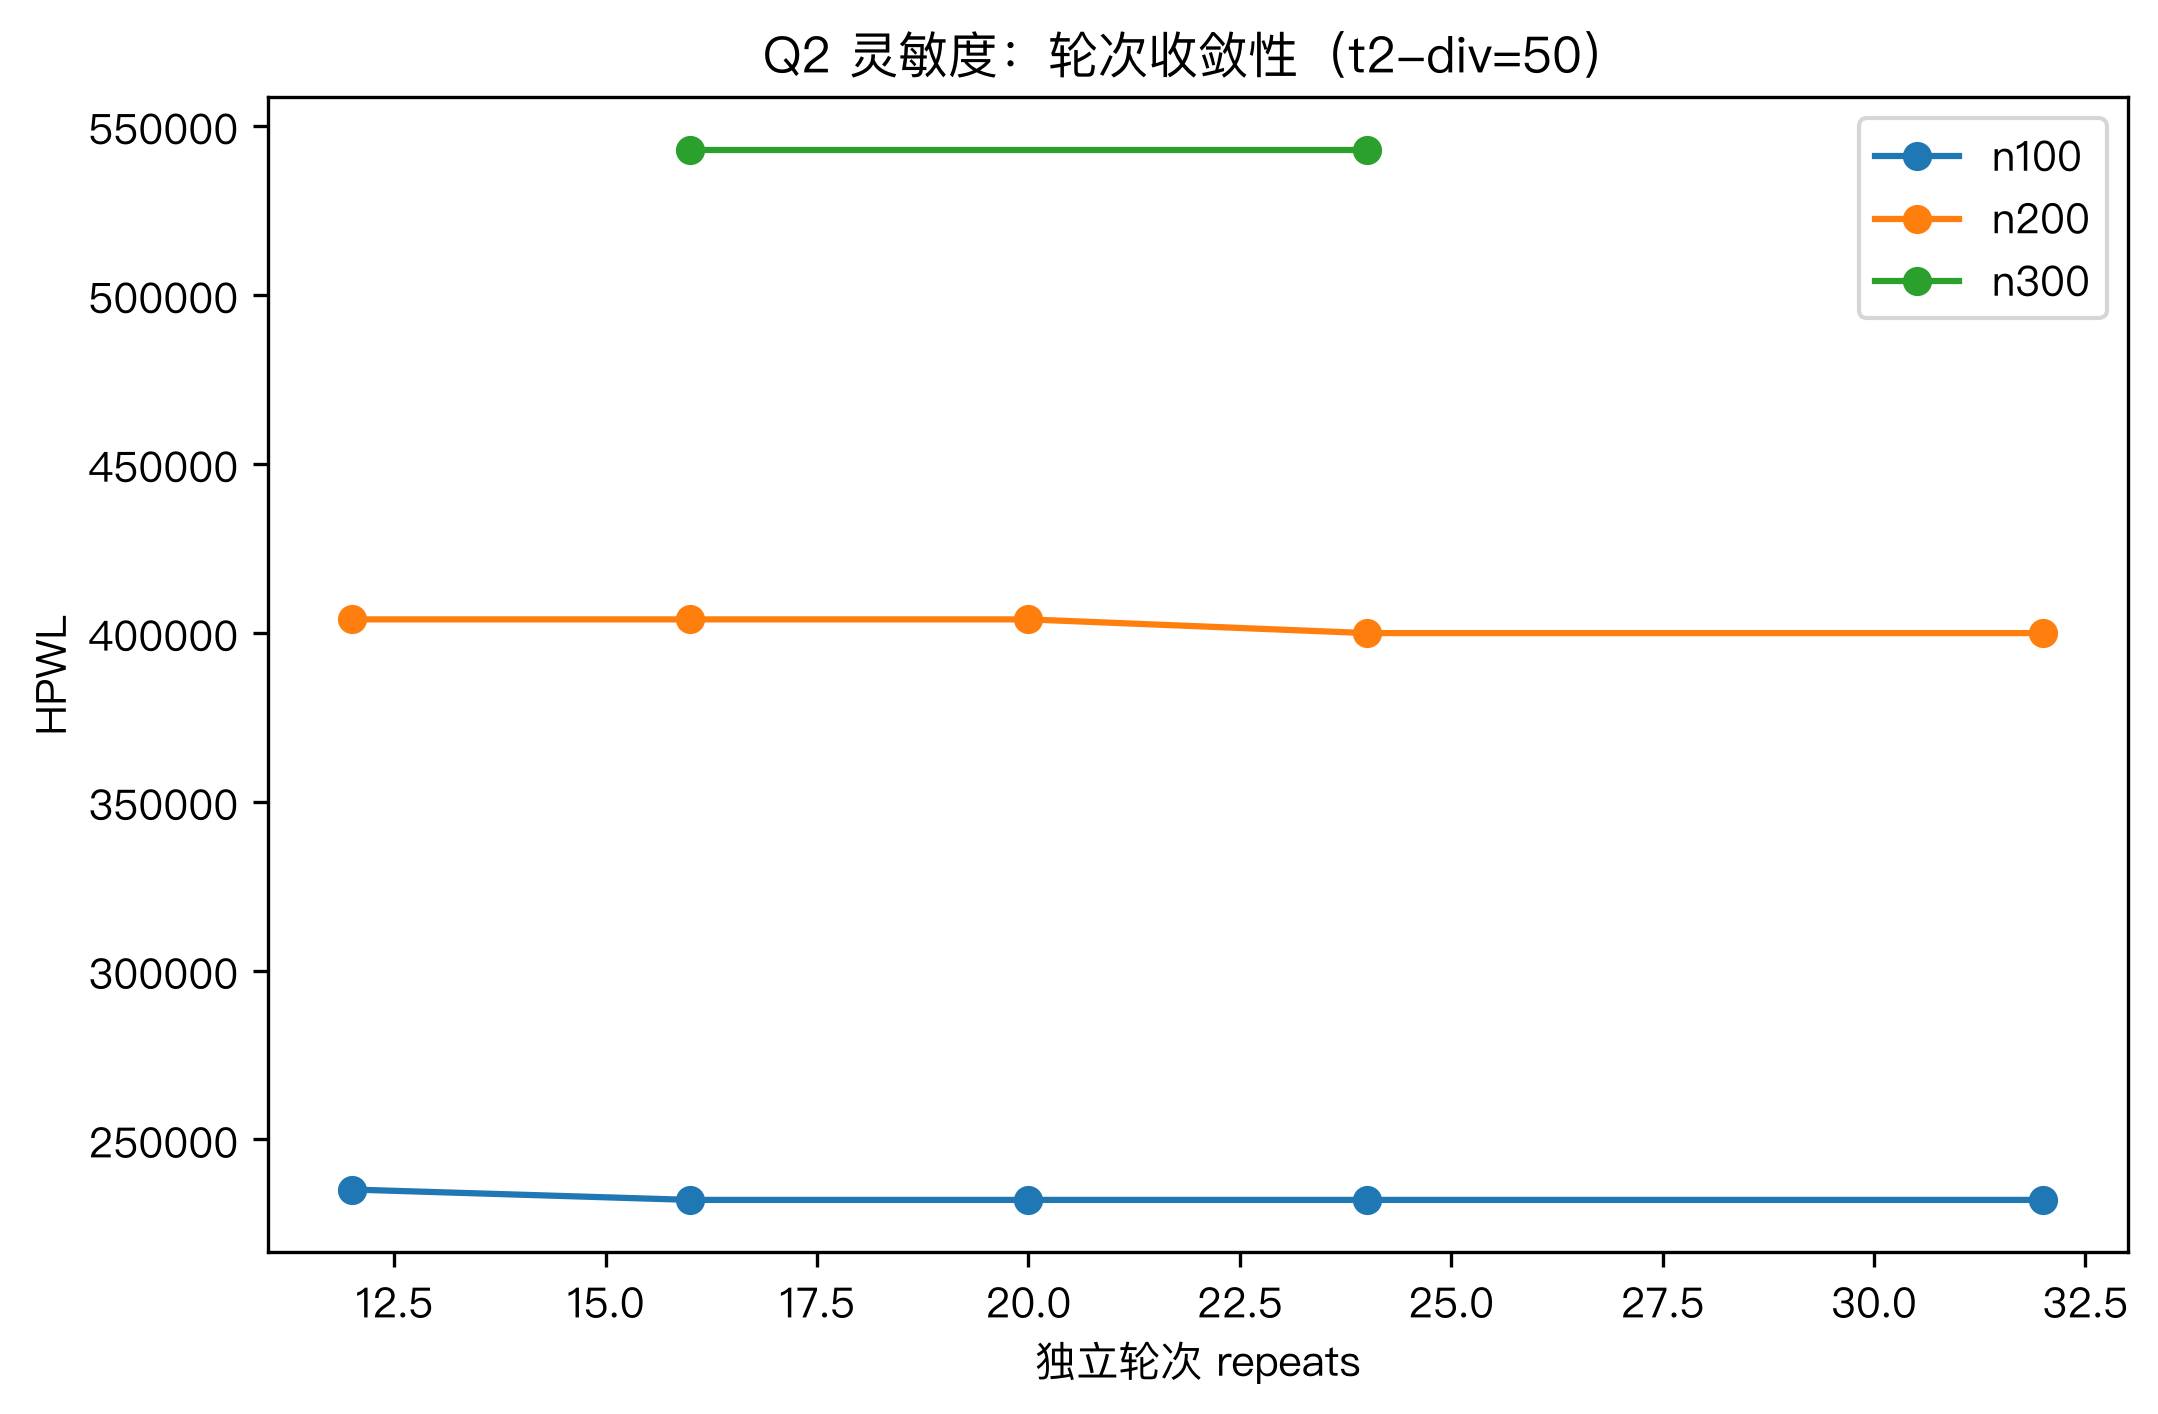
\includegraphics[width=0.82\textwidth]{../../做图/q2_repeats_sensitivity.png}
\caption{HPWL 随独立轮次变化}
\end{figure}

  \begin{table}[H]
  \centering
  \caption{S3 数据}\label{tab:q2s3}
  \begin{tabular}{lll}
  \toprule
  chip & repeats & hpwl \\
  \midrule
  n100 & 12 & 235183.0 \\
  n100 & 16 & 232114.0 \\
  n100 & 20 & 232114.0 \\
  n100 & 24 & 232114.0 \\
  n100 & 32 & 232114.0 \\
  n200 & 12 & 403937.5 \\
  n200 & 16 & 403937.5 \\
  n200 & 20 & 403937.5 \\
  n200 & 24 & 399874.0 \\
  n200 & 32 & 399874.0 \\
  n300 & 16 & 542895.0 \\
  n300 & 24 & 542895.0 \\
  \bottomrule
  \end{tabular}
  \end{table}

\textbf{结论}：n100 在 12 轮后进入平台（225404$\sim$232114 区间）；
n200/n300 在 24$\sim$32 轮仍有小幅改善（约 1$\sim$2\%）。多起点取优
对 Q2 尤其重要——单轮方差极大（见工作稿 8 轮分布表），轮次增加
显著降低 best 的运气成分。

\end{document}
